\documentclass[11pt,letterpaper]{article}
\usepackage{fullpage}
\usepackage[top=2cm, bottom=4.5cm, left=2.5cm, headsep=24pt, right=2.5cm]{geometry}
\usepackage{amsmath,amsthm,amsfonts,amssymb,amscd}
\usepackage{lastpage}
\usepackage{enumerate}
\usepackage{fancyhdr}
\usepackage{mathrsfs}
\usepackage{xcolor}
\usepackage{graphicx}
\usepackage{listings}
\usepackage{booktabs}
\usepackage{amsmath}
\usepackage[utf8]{inputenc}
\usepackage{physics}
\usepackage[colorlinks=true, allcolors=blue]{hyperref}
\usepackage{siunitx}
\usepackage{bm}
\usepackage{float}
\usepackage{subcaption}
\usepackage{tikz}
\usepackage{bm}
\usepackage{hyperref}

\let\oldvec=\vec
\renewcommand{\vec}[1]{\oldvec{\mathbf{#1}}}
\def\doubleunderline#1{\underline{\underline{#1}}}

\def\spvec#1{\left(\vcenter{\halign{\hfil$##$\hfil\cr \spvecA#1;;}}\right)}
\def\spvecA#1;{\if;#1;\else #1\cr \expandafter \spvecA \fi}


\usepackage{fancyhdr}
\pagestyle{fancy}

\newenvironment{qns}[1]
    {\begin{center}
    \begin{tabular}{|p{0.9\textwidth}|}
    \hline
    \begin{center}
        \textbf{#1}\\[1ex]
    \end{center}

    }
    { 
    \\\\\hline
    \end{tabular} 
    \end{center}
    }

\newtheorem{sol}{Solution}[subsection]
  
\newtheorem{thm}{Theorem}

\renewcommand*{\l}{\left(}
\renewcommand*{\r}{\right)}
\newcommand{\partialt}{\frac{\partial}{\partial t}}
\newcommand{\expectation}[1]{\left\langle #1 \right\rangle}
\newcommand{\brakett}[3]{\left\langle#1\left|#2\right|#3\right\rangle}
\newcommand{\partialf}[3]{\frac{\partial^{#3} #1}{\partial #2^{#3}}}
\newcommand{\lbar}{\left|}
\newcommand{\rbar}{\right|}
\renewcommand*{\b}[1]{\mathbf{#1}}
\def\matrix#1{\underline{\underline{#1}}}



\fancyhf{}% Clear header/footer
\fancyhead[C]{Beta 5.0}
\fancyfoot[C]{\thepage}% \fancyfoot[R]{\thepage}
\renewcommand{\headrulewidth}{0.4pt}% Default \headrulewidth is 0.4pt
\renewcommand{\footrulewidth}{0.4pt}% Default \footrulewidth is 0p
\fancyhead[L]{\leftmark}
\fancyhead[R]{\rightmark}

\title{Wavepacket Propagation Program (w/ Dr Nadav Avidor)}
\author{Lorenzo Basso, Jack Lee, Matthew Zhang, Feiyang Chen}
\date{April 2020}

\begin{document}

\maketitle

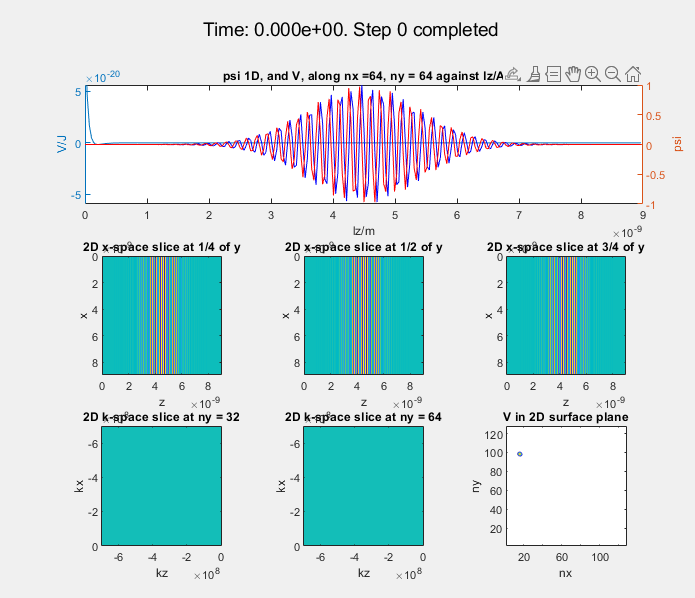
\includegraphics[width = 0.9\textwidth]{Cover.png}


\newpage 
    
\bigskip

\tableofcontents

\newpage

\section{Wavepacket Propagation Introduction}
\subsection{About}

The Wavepacket propagation project is an extension of a Part III project by Ocean Haghighi-Daly. It is a 3D working version of a Working attempt at a Split-Operator method of wavepacket propagation. 


\subsection{Necessary Prerequisites}

To begin with, a computer with a CUDA compatible GPU (\href{https://developer.nvidia.com/cuda-gpus#compute}{List of compatible GPUs}) is required.


\section{Usage}
\subsection{Custom Paths and Potentials}
Functionality to include custom adsorbate paths and potentials was added by Jack Lee.

\begin{enumerate}
    \item Custom potential: this allows you to specify a custom potential profile in the Z direction. To apply this, set decaytype to 4 and specify a .txt file (in beta4\_2) as a string in potfile. This should contain several numbers separated by spaces (or new lines) which are the values for the potential in Joules in each cell of the simulation out from the corrugation function (+zoffset), i.e. the values are separated by a distance of lz/nz. The potential is zero for all z not specified by the file. Zoffset should have a negative value, and can be used to extend the potential back from the gaussians to the surface, as if zoffset is 0 the area between the surface and the gaussian peaks will have 0 potential. The potential specified should be very high near the surface to prevent the wavepacket from getting past it, because the propagation algorithm leads to cyclic boundary conditions so any psi that reaches the end will appear at the other side, which is non-physical.
    \item Custom paths: this allows you to specify the paths that adsorbates take, rather than having them be generated randomly. To enable this, set custompaths to true and specify in pathfile a text file (in beta4\_2) formatted as follows: the first entry on each line should be a time, then for each adsorbate there should be its x position and then its y position at that time, separated by spaces. There can be any number of times, as long as the first is $\leq$ tStart and the last is $\geq$ tFinish, and they’ll be interpolated to get the paths. 
    \item Saving paths: this allows you to save the randomly generated paths adsorbates take this time in the simulation. It doesn’t do anything if custom paths is on. To enable it, set savingBrownianPaths to true and name a .txt file in Browniefile, which will be overwritten or created in beta4\_2. This saves the paths in the same format as Custom paths reads them, with one line for each timestep of the simulation. These files can later be read by custom paths to reproduce this simulation (and could be used to vary the potential, detail etc.), although there is a small error introduced here so that the final psi from the custom paths simulation is slightly different to that of the original. Two custom paths simulations from the same source will be the same, however.
\end{enumerate}


\end{document}
